
\section{Appendix}\label{sec:appendix}


\subsection{Activation function}
\noindent The function $\Phi_{\cdot}$ is defined by combining a generalized version of the sigmoid, namely with a gain $\beta \neq 1$ and offset $\alpha\neq 0$, and a Gaussian with mean $\mu$ and variance $\sigma$. Their contributions are weighted by as $r$ and $1-r$ ($r\in(0,1)$) respectively.

\begin{equation*}
    \Phi_v(x) = r\left(1 + \exp^{-\beta(x-\alpha)}\right)^{-1} + (1-r)\exp\left(-\frac{(x-\mu)^2}{2\sigma^2}\right)
\end{equation*}

\noindent The motivation behind this choice is to express a function that possesses a bounded region (depending on $\mu,\,\sigma$) at a high/low peak (depeding on the value of $\gamma_{2}$), and a continuous transition to a constant value (depending on the steepness of the sigmoid $\beta$, shift
$\alpha$, and intensity $\gamma_{1}$).

\begin{figure}[ht]
    \centering
    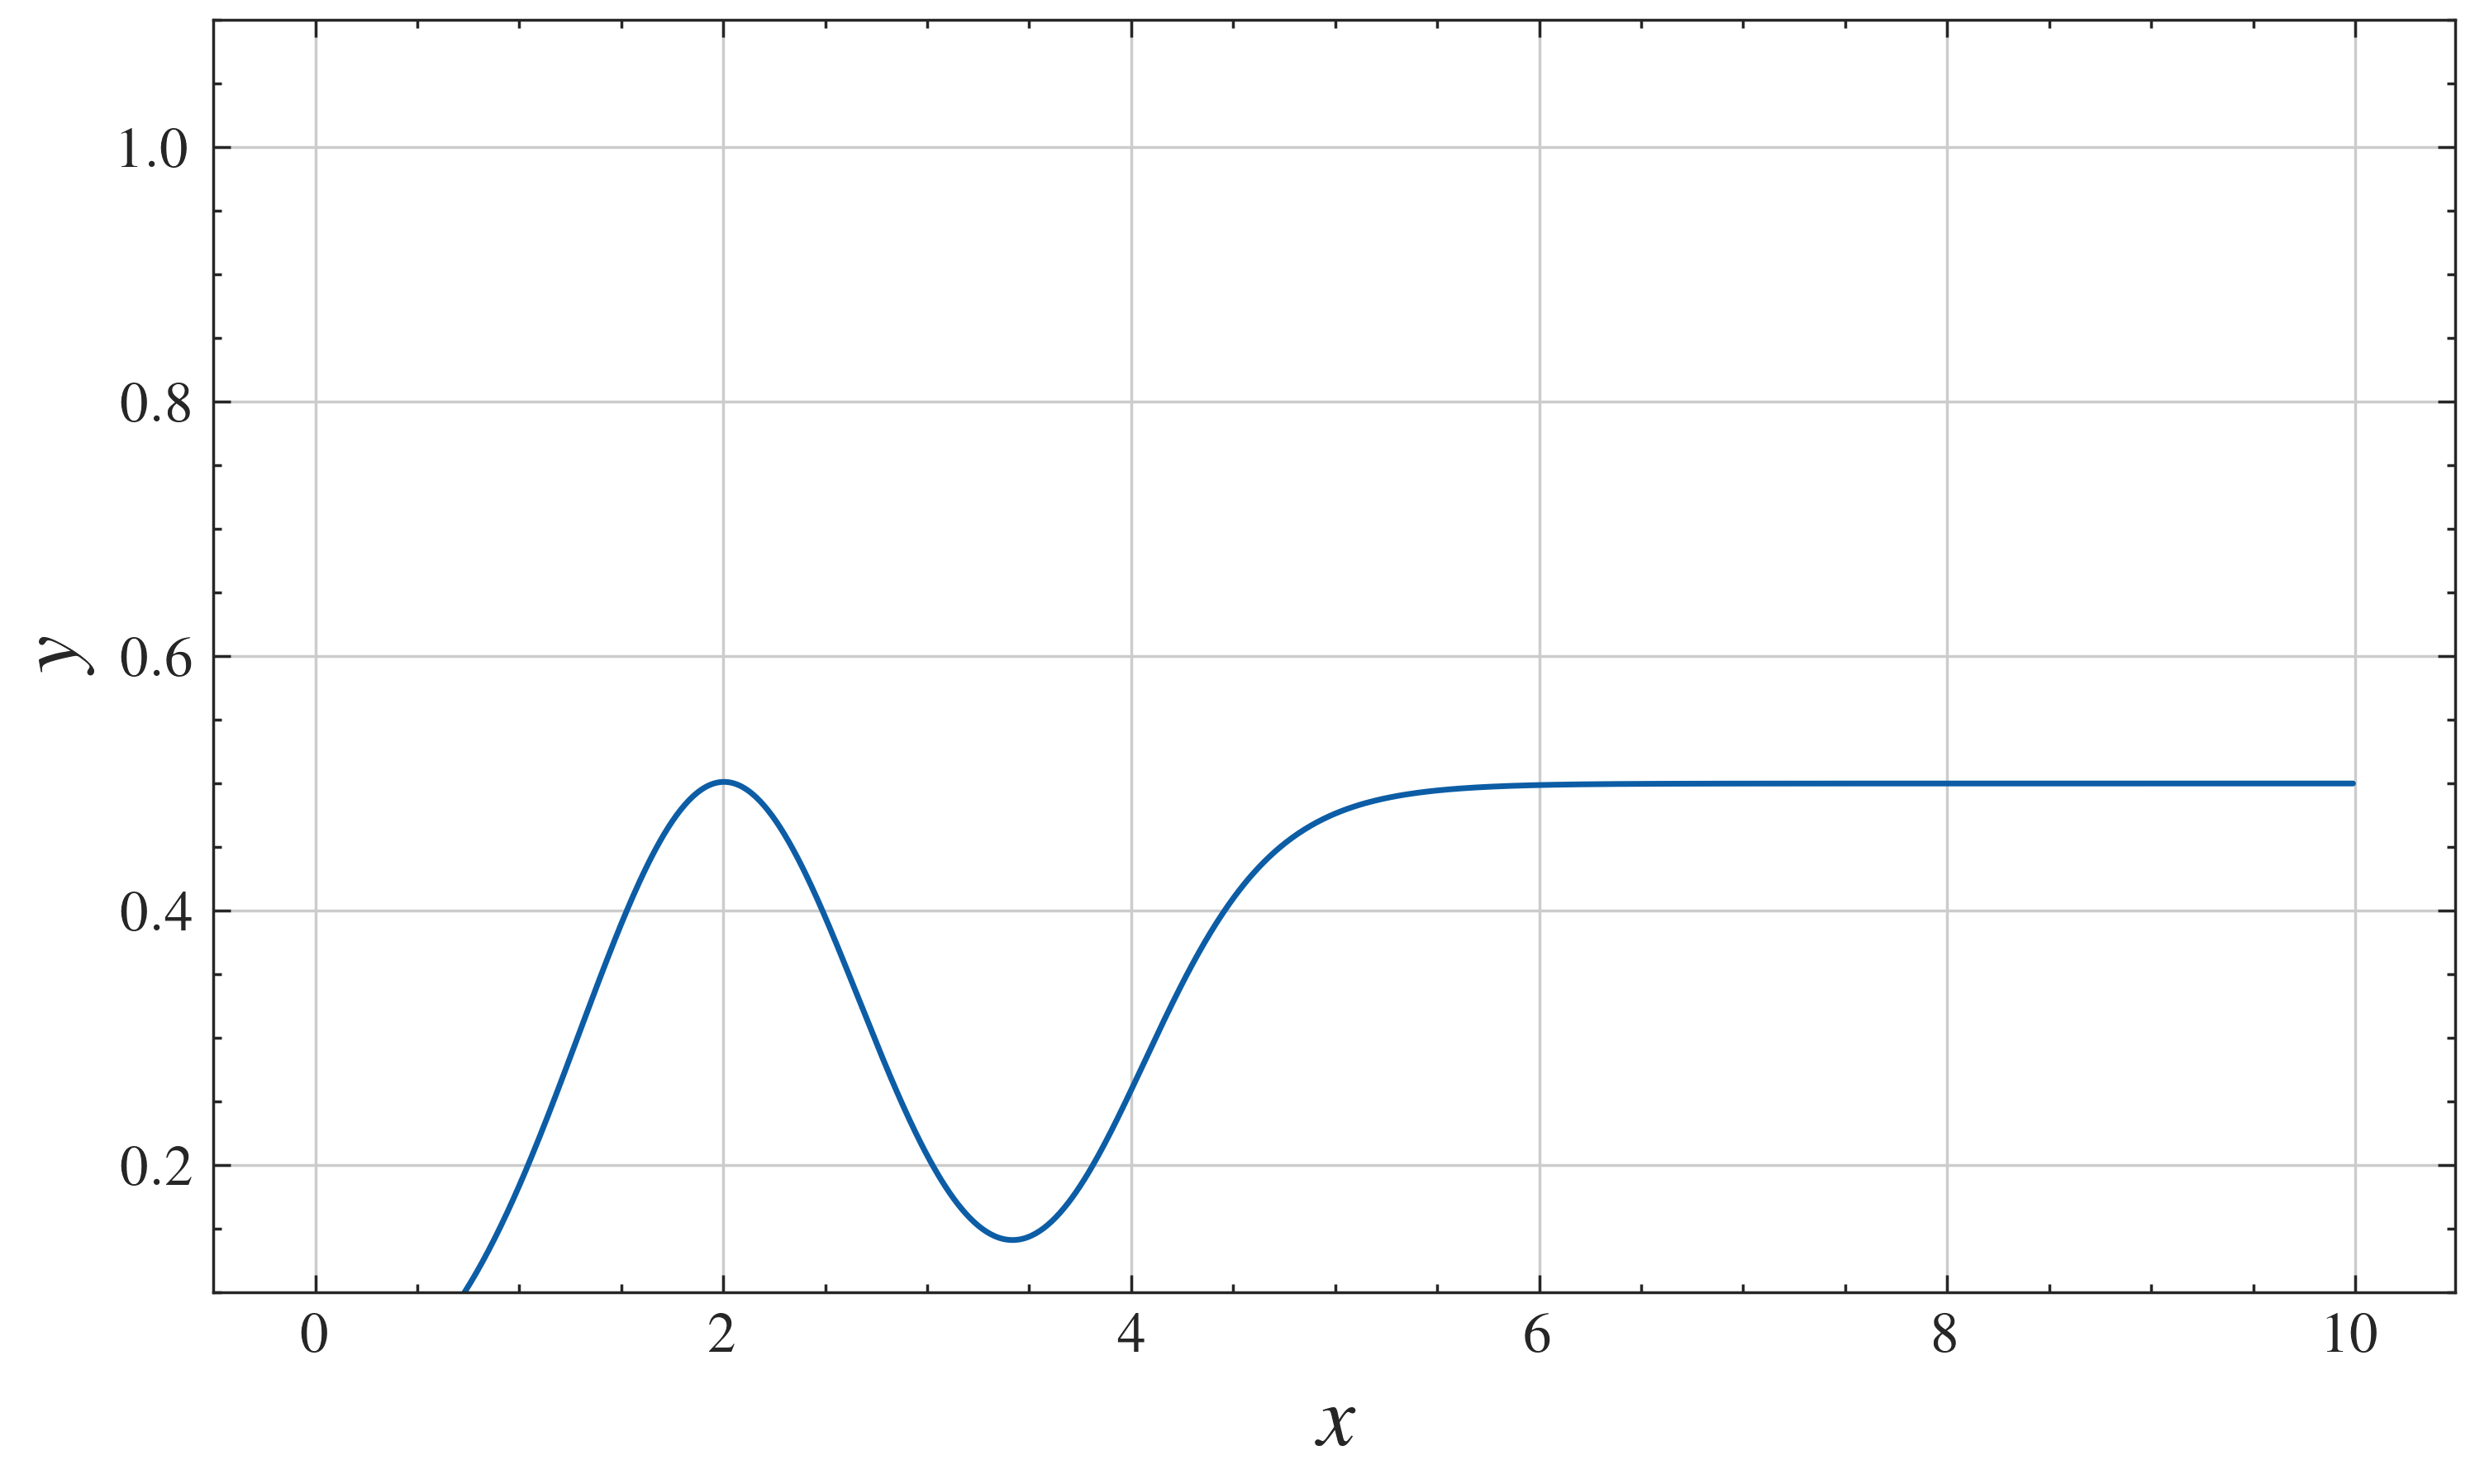
\includegraphics[width=0.8\textwidth]{figures/gaussian_sigmoid.png}
    \caption{\textsc{Activation function $\Phi_{v}$} - \textit{Parameters $\beta=10$, $\alpha=1$, $\mu=1$, $\sigma=1$, and $r=0.5$.}}
    \label{fig:gau_sigm}
\end{figure}

\subsection{Zero-steps distribution shift}
In this first setting, as the end of a trial $i$ the arm distribution changes immediately to a new one $i+1$ as $\mathbf{\pi}_{i} \to \mathbf{\pi}_{i+1}$.

\begin{figure}[ht]
    \centering
    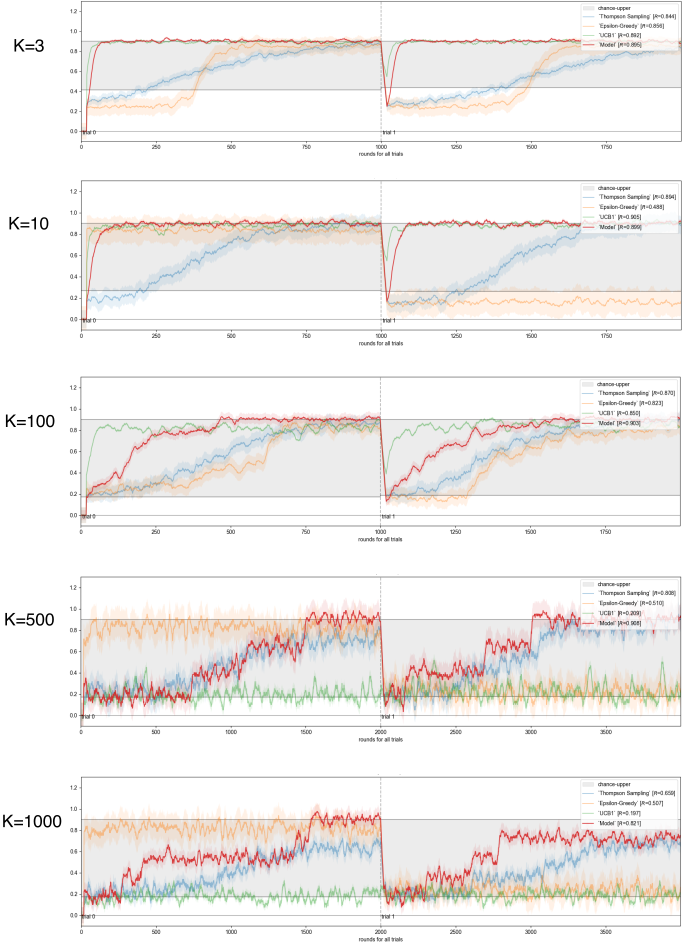
\includegraphics[width=0.65\textwidth]{figures/drawing.png}
    \caption{\textsc{Performance with variable number of arms} - \textit{each plot is a simulation with K numbers of arms, the x-axis are rounds, the central vertical line signals the start of the second trial, the y-axis is the reward fraction.
            The shaded area is the reasonable reward
    range, where the lower bound is the chance level and the upper bound the best reward (following the optimal policy). The model performance is in red, while Upper-Confidence Bound green, Thompson Sampling blue, and Epsilon-Greedy orange. }}
\label{fig:zero_1}
\end{figure}


\noindent From figure \ref{fig:zero_1} above, it is clear the ability of the model (in red) to reach almost always the optimal reward policy (\textit{i.e.} the greediest) for all trials, even after the distribution shift.
In comparison, the other algorithms start to struggle when the arms are more $100$ and the distribution changes.

Next, it has been enquired how the model selection policy evolves over time and in comparison with the other algorithms, as visualized in figure \ref{fig:sel2}.

\begin{figure}[ht]
    \centering
    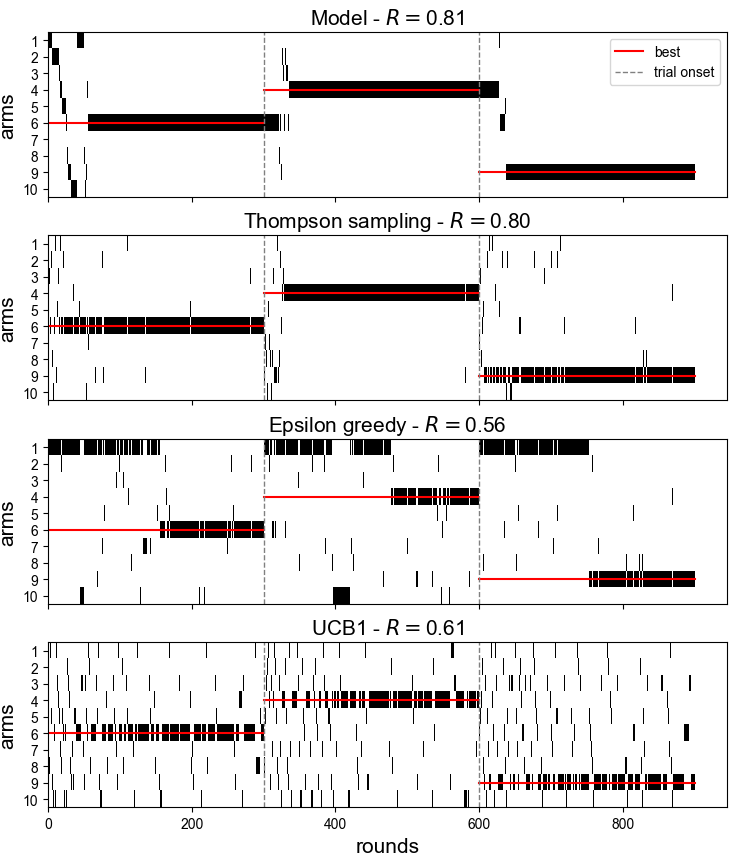
\includegraphics[width=0.9\textwidth]{figures/selections_many.png}
    \caption{\textsc{Selection evolution over rounds for multiple models} - \textit{the individual plots follow the same schema of \ref{fig:sel1}, with the model name and reward per round fraction}}
    \label{fig:sel2}
\end{figure}

\noindent The principal distinction is the model's strictly greedy behaviour once a good arm is found. Only in the case of a meaningful decrease in reward the exploration is resumed, in contrast with the other approaches in which occasional sub-optimal choices are made.


\subsection{Epsilon-steps distribution shift}

\begin{figure}[ht]
    \centering
    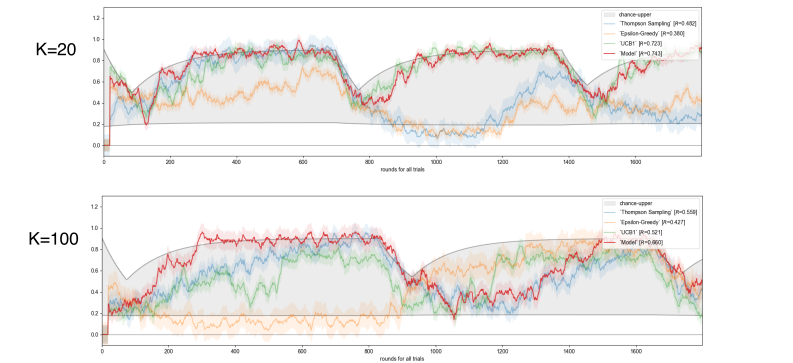
\includegraphics[width=0.8\textwidth]{figures/drawing2.png}
    \caption{\textsc{Performance with variable number of arms} - \textit{each plot is a simulation with K-numbers of arms, and the rest is also the same as before in \ref{fig:zero_1}}. Each trial has 3 rounds, meaning that every three steps the distribution change.}
    \label{fig:eps_1}
\end{figure}

\noindent In the setting with a smooth distribution shift the difficulty of the problem is increased, especially since short-sighted greedy behaviours are easily sub-optimal. The model (always in red) is capable of reaching and maintaining a successful profile, even with many arms available.


\subsection{Table of results}

% --- table K.5
\begin{table}[H]
\centering
\caption{Performance comparison for $K=5$}
\label{tab:k5}
\begin{tabular}{l c c c}
\toprule
\textbf{Model} & \textbf{\textsc{KAB-0}} & \textbf{\textsc{KAB-$\epsilon$}} & \textbf{\textsc{KAB-$\sin$}}\\
\midrule
Optimal & $0.900$ & $0.881$ & $0.563$ \\
Random & $0.330$ & $0.337$ & $0.200$ \\
\midrule
Thompson & $0.905$ & $0.617$ & $0.317$ \\
$\epsilon$-Greedy & $0.797$ & $0.531$ & $0.315$ \\
UCB & $0.897$ & $0.656$ & $0.319$ \\
\textbf{Model} & $\mathbf{0.899}$ & $\mathbf{0.663}$ & $\mathbf{0.265}$ \\

\bottomrule
\end{tabular}
\end{table}

% --- table K.10
\begin{table}[H]
\centering
\caption{Performance comparison for $K=10$}
\label{tab:k10}
\begin{tabular}{l c c c}
\toprule
\textbf{Model} & \textbf{\textsc{KAB-0}} & \textbf{\textsc{KAB-$\epsilon$}} & \textbf{\textsc{KAB-$\sin$}} \\
\midrule
Optimal & $0.900$ & $0.885$ & $0.355$  \\
Random & $0.247$ & $0.250$ & $0.100$ \\
\midrule
Thompson & $0.896$ & $0.648$ & $0.339$ \\

$\epsilon$-Greedy & $0.611$ & $0.597$ & $0.343$ \\
UCB & $0.891$ & $0.655$ & $0.358$ \\
\textbf{Model} & $\mathbf{0.905}$ & $\mathbf{0.668}$ & $\mathbf{0.203}$  \\
\bottomrule
\end{tabular}
\end{table}

% --- table K.100
\begin{table}[H]
\centering
\caption{Performance comparison for $K=100$}
\label{tab:k100}
\begin{tabular}{l c c c}
\toprule
\textbf{Model} & \textbf{\textsc{KAB-0}} & \textbf{\textsc{KAB-$\epsilon$}} & \textbf{\textsc{KAB-$\sin$}} \\
\midrule
Optimal & $0.900$ & $0.883$ & $0.020$  \\
Random & $0.196$ & $0.201$ & $0.010$ \\
\midrule
Thompson & $0.894$ & $0.586$ & $0.013$ \\
$\epsilon$-Greedy & $0.519$ & $0.574$ & $0.018$ \\
UCB & $0.853$ & $0.572$ & $0.012$ \\
\textbf{Model} & $\mathbf{0.898}$ & $\mathbf{0.651}$ & $\mathbf{0.010}$  \\
\bottomrule
\end{tabular}
\end{table}

% --- table K.200
\begin{table}[H]
\centering
\caption{Performance comparison for $K=100$}
\label{tab:k200}
\begin{tabular}{l c c c}
\toprule
\textbf{Model} & \textbf{\textsc{KAB-0}} & \textbf{\textsc{KAB-$\epsilon$}} & \textbf{\textsc{KAB-$\sin$}} \\
\midrule
Optimal & $0.900$ & $0.885$ & $0.010$  \\
Random & $0.178$ & $0.176$ & $0.005$ \\
\midrule
Thompson & $0.875$ & $0.624$ & $0.006$ \\
$\epsilon$-Greedy & $0.679$ & $0.588$ & $0.010$ \\
UCB & $0.792$ & $0.510$ & $0.006$ \\
\textbf{Model} & $\mathbf{0.905}$ & $\mathbf{0.610}$ & $\mathbf{0.006}$  \\
\bottomrule
\end{tabular}
\end{table}

% --- table K.1000
\begin{table}[H]
\centering
\caption{Performance comparison for $K=100$}
\label{tab:k1000}
\begin{tabular}{l c c c}
\toprule
\textbf{Model} & \textbf{\textsc{KAB-0}} & \textbf{\textsc{KAB-$\epsilon$}} & \textbf{\textsc{KAB-$\sin$}} \\
\midrule
Optimal & $0.900$ & $0.880$ & $0.002$  \\
Random & $0.177$ & $0.178$ & $0.001$ \\
\midrule
Thompson & $0.779$ & $0.445$ & $0.001$ \\
$\epsilon$-Greedy & $0.386$ & $0.478$ & $0.002$ \\
UCB & $0.301$ & $0.185$ & $0.001$ \\
\textbf{Model} & $\mathbf{0.703}$ & $\mathbf{0.480}$ & $\mathbf{0.001}$  \\
\bottomrule
\end{tabular}
\end{table}


\newpage
